\chapter{Music Playlist Shuffling}\label{final}
Since our recommendation system runs very frequently(every hour or every day), it is necessary for the recommendation system to re-score the available items at every period of time. let's say we have a time period of T then after every time period the item list should have some changes. But in this period the user will get the same list of items. in today's time user can get bored if he/she sees the same content every time he/she opens the application during the period T.There can be many ways this scenario can happen but imagine the user opens the application and doesn't like the recommended items and is too lazy or busy to scroll or search for something else.If the user opens the application again some minutes later to find exactly the same content as before this might have a big (negative) impact on the retention for this user.

\section{Shuffling}
One solution to this problem is to shuffle the content of the playlist in such a way that it remains
relevant to the user. After shuffling, the list can have some new items but in a different order.
we can use shuffling in two ways- One is that we have a large playlist(size m) of items and we shuffle the whole playlist and show top-n out of m items.Here after every time some items can change its order and some new items can also appear in top-n list. Another way is that we can have a playlist of size n and we shuffle the whole list and show all the items of the list.Here no new item will appear but the order of the items will be changed.

Here are the types of shuffling we use

\subsection{Fisher-Yates Shuffle}

The assumption here is, we are given a function rand() that generates random number in O(1) time.The idea is to start from the last element, swap it with a randomly selected element from the whole array (including last). Now consider the array from 0 to n-2 (size reduced by 1), and repeat the process till we hit the first element.Fisher–Yates shuffle Algorithm works in O(n) time complexity.


\textbf{How does this work?}
The probability that ith element (including the last one) goes to last position is 1/n, because we randomly pick an element in first iteration.

The probability that ith element goes to second last position can be proved to be 1/n by dividing it in two cases.

\textbf{Case 1}: i = n-1 (index of last element):
The probability of last element going to second last position is = (probability that last element doesn’t stay at its original position) x (probability that the index picked in previous step is picked again so that the last element is swapped)
So the probability = ((n-1)/n) x (1/(n-1)) = 1/n

\textbf{Case 2:} 0 < i < n-1 (index of non-last):
The probability of ith element going to second position = (probability that ith element is not picked in previous iteration) x (probability that ith element is picked in this iteration)
So the probability = ((n-1)/n) x (1/(n-1)) = 1/n




\textbf{pseudo code}:

     Choose i = from last index of the list to first index of the list:
     
     choose j = Random value among 0 to ith index:
     swap(value at i th index, value at j th index

Fisher-Yates algorithm for shuffling chooses one index randomly and one index linearly from last position to first position and swap the elements of these two positions.


\begin{figure}
\centering
\begin{subfigure}
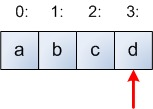
\includegraphics[scale=.5]{report/fy1.jpeg}
\label{chap3Fig:1}
\end{subfigure}
\begin{subfigure}
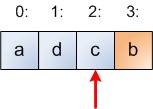
\includegraphics[scale=.5]{report/fy2.jpeg}
\end{subfigure}
\begin{subfigure}
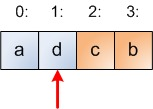
\includegraphics[scale=.5]{report/fy3.jpeg}
\end{subfigure}
\begin{subfigure}
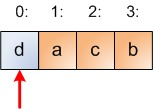
\includegraphics[scale=.5]{report/fy4.jpeg}
\end{subfigure}
\begin{subfigure}
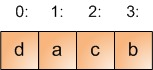
\includegraphics[scale=.5]{report/fy5.jpeg}
\caption{Fisher Yates}
\end{subfigure}
\end{figure}



\begin{figure}
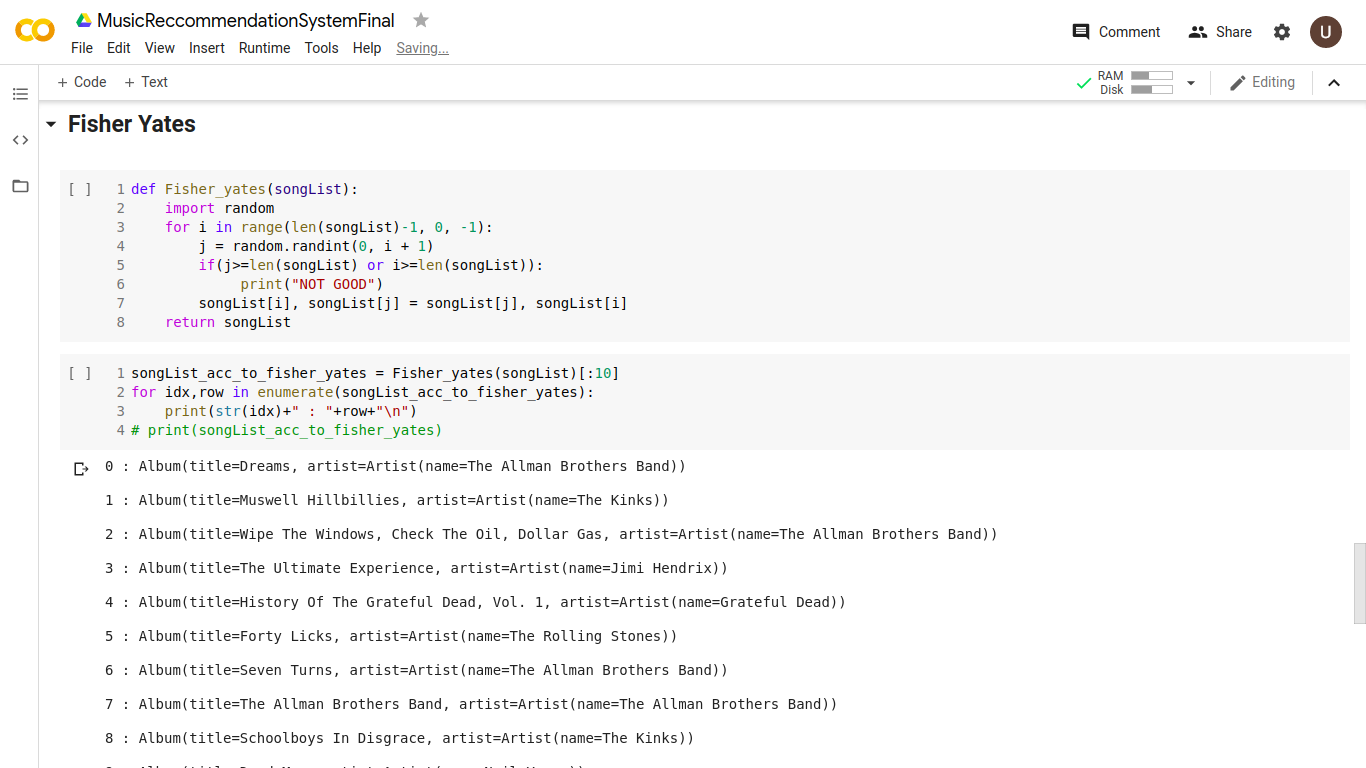
\includegraphics[scale=.5]{report/Fisheryates.png}
\caption{Flow Chart}
\label{chap0Fig:2}
\end{figure}





\subsection{Etilist Shuffle}
This is a very simple approach, In this method of shuffling, every item has given some weight then we calculate weighted probability. Items will be chosen for shuffling based on its weighted probability.

(this is the same as sampling from a multinomial distribution without replacement)

A parameter called inequality is introduced as a knob to tune the weight probability difference between positions.
maximum probability remains on the initial positions in the Etilist Shuffle, Probability decays monotonically with the distance from the initial position, higher ranked items have a higher chance of  being moved from their initial position.

\textbf{Importance of inequality:} If we want higher items to be more probable to remain on top position we'll increase inequality value.

\textbf{features: } 

1. The maximum probability remains on the initial position.

2. Probability decays monotonically with the distance from the initial position.

3. The distribution is non-symmetrical but smoother than the previous example.

4. A big win is that the inequality parameter has a direct understandable impact on the resulting distributions, want higher items to be more probable to remain on top? Increase inequality. In addition, the behavior translates into the desired functionality:

5. Top content would still be relevant after shuffle.
Content is not the same.
Some content has changed position.

\textbf{Drawback:}

The elitist shuffle function is much slower than np.random.shuffle, but still fast for a common application. Considering scenario where the items to shuffle are 100, the elitist shuffle function takes around 1.8ms.



\begin{figure}
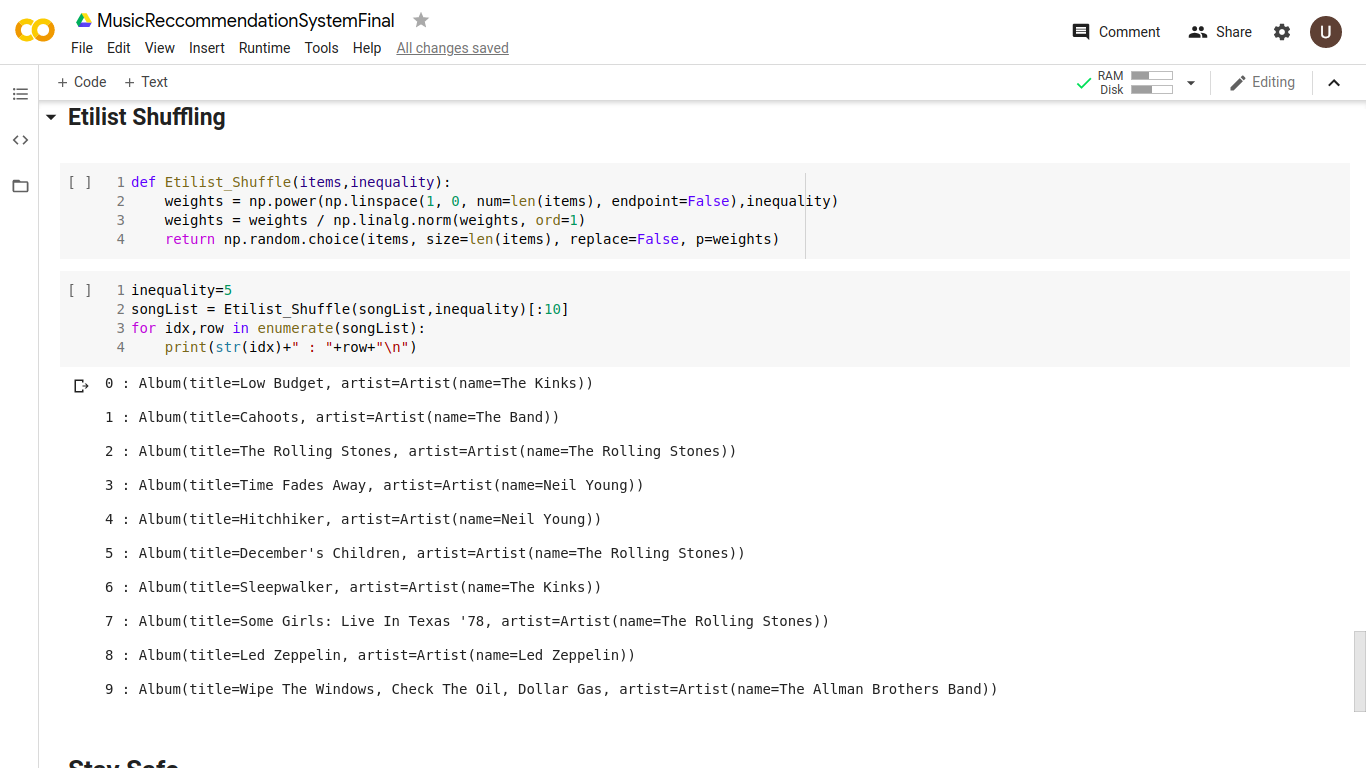
\includegraphics[scale=.5]{report/EtilistShuffing.png}
\caption{Flow Chart}
\label{chap0Fig:2}
\end{figure}



\begin{figure}
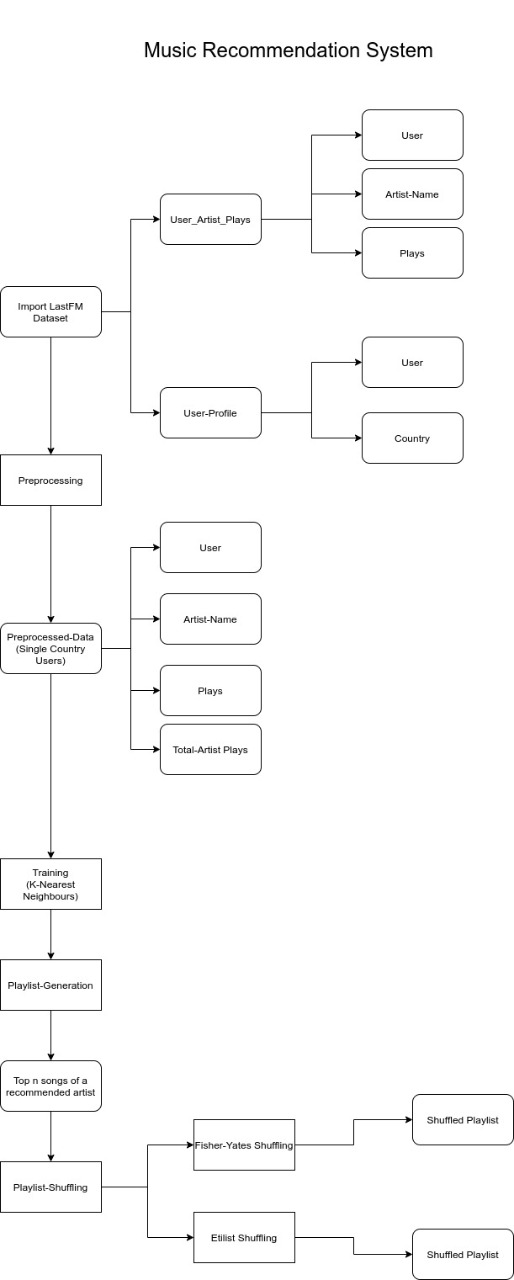
\includegraphics[scale=.5]{report/flowchar.jpeg}
\caption{Flow Chart}
\label{chap0Fig:2}
\end{figure}